\StartPlate{V19}{Abstract actions and native normalizers}{Abstract lifting and arithmetic realization are different existence statements.}
\begin{center}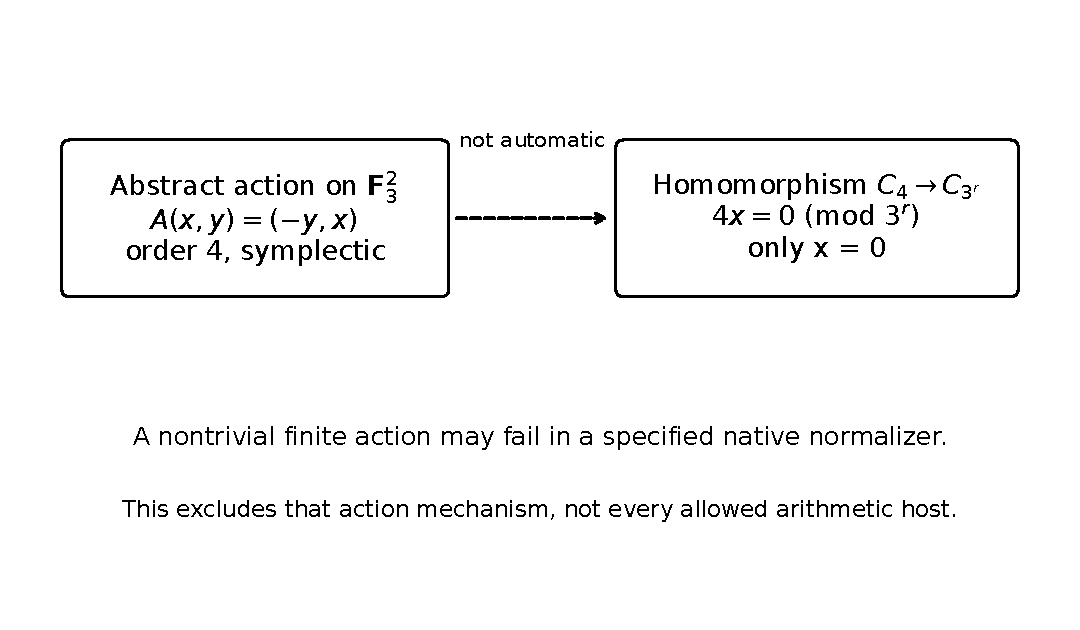
\includegraphics[width=\linewidth]{figures/V19.pdf}\end{center}
The linear map $A(x,y)=(-y,x)$ on $\F_3^2$ is symplectic and has order four. Thus there is a genuine nontrivial abstract $C_4$ action. In contrast, every homomorphism $C_4\to C_{3^r}$ is trivial: an image $x$ satisfies $4x=0$, and multiplication by four is invertible modulo $3^r$.

The arithmetic obstruction uses its stated native-normalizer quotient and inner-action requirements. When that permitted quotient is a $p$-group, a prime-to-$p$ subgroup cannot implement the desired nontrivial action through it. The cyclic groups in the drawing isolate the elementary coprimality mechanism. They are not asserted to be the entire normalizer of every type.

Finite central-extension actions can still lift under their own coprimality hypotheses, and projective intertwiners can sometimes be linearized. Neither result supplies the missing arithmetic conjugating matrices. An obstruction to this normalizer mechanism therefore remains compatible with success through a different allowed host or a different stated attachment contract.
\vfill\PlateSource{Exact coprimality analogue}{Part I, Sections 4 and 11}{9}
